
\documentclass[10pt,twocolumn,letterpaper]{article}

\usepackage{cvpr}
\usepackage{times}
\usepackage{epsfig}
\usepackage{graphicx}
\usepackage{amsmath}
\usepackage{amssymb}
\usepackage{enumerate}
\usepackage[breaklinks=true,bookmarks=false]{hyperref}

\cvprfinalcopy % *** Uncomment this line for the final submission

\def\cvprPaperID{****} % *** Enter the CVPR Paper ID here
\def\httilde{\mbox{\tt\raisebox{-.5ex}{\symbol{126}}}}
\setcounter{page}{1}
\begin{document}

\title{MemGAN: Increasing Memorability of Images using GANs}

\author{Akarsh Zingade\\
{\tt\small auz2000@columbia.edu}
\and
James Shin\\
{\tt\small js4785@columbia.edu}
\and
Aashish Misraa\\
{\tt\small akm2215@columbia.edu}
}

\maketitle



% \name{ Akarsh Zingade, Aashish Misraa, James Shin }

% \address{ \{auz2000@columbia.edu, akm2215@columbia.edu, js4785@columbia.edu\}\\}





% \maketitleabstract

\textbf{Abstract.} \textit{Humans are great at remembering thousands of images and even specific parts of these images despite the high overflow of visual information. The degree to which an image is remembered is known as Image Memorability. Prior research \cite{memo} has shown that image memorability can be quantified and measured. Other works have shown that memorability can be estimated with machine learning frameworks, initially with low-level, global image features \cite{photo_mem}, and deep learning \cite{image_mem_deep, mem_pred_bias, adap_transf} approaches. Once we have estimated the memorability of an image, is it possible to manipulate the image to increase the memorability of the image? Prior work \cite{photo,style,face} have had some success in doing so. In this work, we use Generative Adversarial Networks to increase the memorability of the image using CityScapes dataset. First, we propose a new objective function that introduces memorability. Second, we propose an evaluation method to show that the network indeed benefits from the proposed objective function. Third, we show that a model trained using the proposed memorability loss can increase the memorability of an image by 20\% on average. Lastly, Human opinion studies demonstrate that our method significantly outperforms existing methods, advancing both the quality and the resolution of deep image synthesis and editing.}

%%%%%%%%%%%%%%%%%%%%%%%%%%%%%%%%%%%%%%%%%%%%%%%%%%%%%%%%%%%%%%%%%%%%%%%%


\section{Introduction}



\section{Review of Prior Work}
% There have been significant works on the topic of image memorability. 
Isola et al. \cite{memo} was the first to attempt to quantify image memorability. A restricted experimental setting was used to measure memorability of an image. They defined memorability as the probability that a viewer will detect repeated images when he is shown a series of pictures. They also showed that predicting an image's memorability could be achieved through classical computer vision techniques. \cite{lamem} used an experimental setting to collect memorability scores on many images and built a dataset called LaMem based on those scores. This dataset consists of 60,000 images, making it the largest annotated image memorability dataset. We plan on training our memorability predictor on LaMem. \\

% The experimental setup that they used to determine this includes observer pressing the key when shown the images seen before. They rank the images in such a way that they account for varied time intervals allowing them to obtain high consistency with existing benchmarks. 


From our knowledge, there have been three works on increasing memorability- using style transfer \cite{style}, changing face photographs \cite{photo}, and editing attributes of the face \cite{face}.
\cite{face} uses CelebA \cite{celeb}, consisting of 200K images, to create synthetic labels using a predictor trained on 2K images with scores collected from \cite{iso}.
They use a Generative Adversarial Network (GAN) \cite{gene}, which is a generative model consisting of a generator $G$ to model the data distribution, and a discriminator $D$ to discriminate samples generated from $G$ and the training set. From a prior distribution $p_z(z)$ the generator learns to map it to a data space.
The value function for the two player min-max game is:
\begin{align*}
    \min_{G}\max_{D}V(D,G) &= \mathbb{E}_{x \stackrel{}{\sim} p_{data}}[\text{log} D(x)] \\
    &+ \mathbb{E}_{z \stackrel{}{\sim} p_z(z)} [\text{log}(1 - D(G(z)))]
\end{align*}

In \cite{face}, AttGAN \cite{attgan} is used to conditionally generate new images by considering memorability as an attribute while preserving other facial attributes. Another approach to increase memorability previously used is style transfer \cite{style} where they use a deep architecture for generating a picture that is memorable from a input image and a style seed. They rely on deep models and a learning-based solution to automatically select the best style also.
\\

Our plan is to design a novel way of making images more memorable while allowing the ability to add objects to the image while maintaining (or increasing) the memorability. We plan to leverage previous works in the domain of image-to-image translation and generative adversarial networks.  Pix2Pix \cite{pix2pix} uses a conditional GAN \cite{cgan} which has a UNet-based generator \cite{unet}, and the discriminator is a convolutional PatchGAN classifier, which only penalizes structure at the scale of image patches. Pix2Pix fails to scale to high resolution images. Pix2PixHD builds on Pix2Pix to generate high-resolution images using a multi-scale generator and discriminator. Pix2PixHD estimates the semantic map of the input image, to allow the manipulation of the semantic information, and then synthesizes a natural image using the edited semantic information. This makes the manipulation of objects very easy. Therefore, the user is able to manipulate and synthesize natural images. The dataset that we will use to train this Pix2PixHD is cityscapes \cite{city}. Cityscape comprises of diverse, large set of stereo sequences of video recorded in streets of 50 different cities. In this dataset, 5K images have high quality pixel-level annotation and 20K additional image with coarse annotations. These peculiarities of this dataset makes it very suitable for pixel-level, instance-level semantic labeling or weakly-supervised learning.

%%%%%%%%%%%%%%%%%%%%%%%%%%%%%%%%%%%%%%%%%%%%%%%%%%%%%%%%%%%%%%%%%%%%%%%%

\begin{figure}
    \centering
    \label{pic1}
    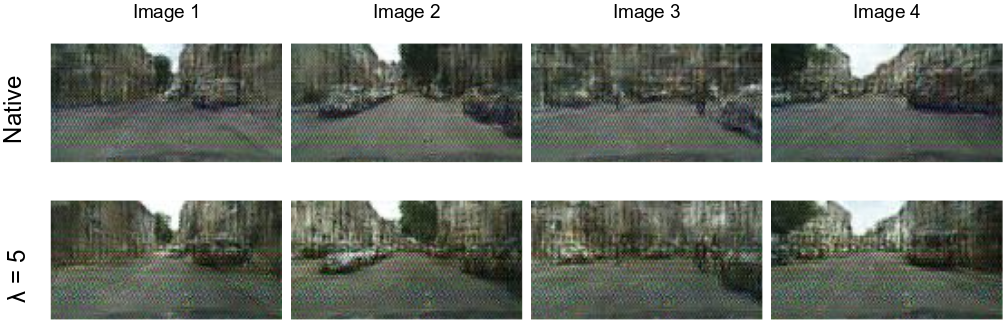
\includegraphics[width=\linewidth]{pic1.png}
    \caption{\textit{Showing stuff}}
\end{figure}

\begin{figure}
    \centering
    \label{pic2}
    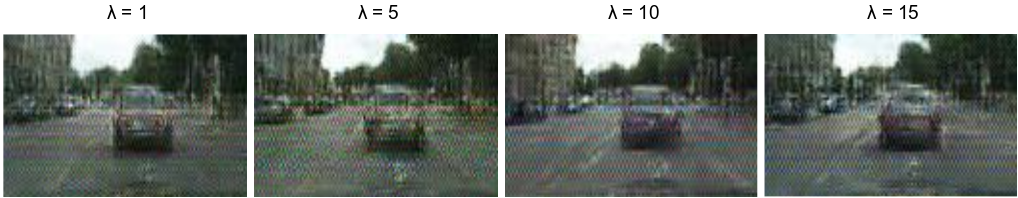
\includegraphics[width=\linewidth]{pic2.png}
    \caption{\textit{Showing stuff}}
\end{figure}

%%%%%%%%%%%%%%%%%%%%%%%%%%%%%%%%%%%%%%%%%%%%%%%%%%%%%%%%%%%%%%%%%%%%%%%%


\section{Methodology}
The Pix2PixHD architecture has the general structure shown in 
Before building on the Pix2PixHD architecture, we deci
On top of the Pix2PixHD network, we introduced our own memorability loss function. By leveraging the generator present in Pix2PixHD, the modified network would learn to output images with increased memorability. The memorability loss is defined as the following:
$$ \left(\text{max} \left\{ 0, \text{min} \left\{ 1, M_O + G \right\} - M_F \right\} + L_2 \left(1, M_F \right) \right) * \lambda $$
where $G$ is the 'gap parameter', and $M_O$ and $M_F$ are the memorabilities of the original and fake images respectively, ranging from 0 to 1. Memorability scores $M_O$ and $M_F$ are given by a separate network called 'AMNet', which we discuss in further depth in Section \ref{amnet_section}. The intuition is to increase the memorability of the fake image over each epoch by at least the gap parameter $G$. We cap $M_O + G$ at 1, and try to maximize its value over $M_F$. We also add a simple $L_2$ loss of $M_F$ with 1 in order to increase memorability of the fake images over time. This loss is added in addition to the other losses present in the Pix2PixHD network. In order to weigh its influence relative to other losses, we introduce a scale parameter $\lambda$; we use several values of $\lambda$ in our experiments and show results in Section \ref{results_section}.\\
\indent We also introduced a memorability penalization term to the network. We noticed that many images in the CityScapes dataset

\section{Implementation}

\section{Evaluation Metrics}
We divide this section into two parts. One to show how the memorability of an image is evaluated. The other to evaluate the impact of the memorability loss.
\subsection{Memorability regression network or AMNet mem score}
\label{amnet_section}
\subsection{Comparing to native}
While Pix2PixHD performs extremely well in  generating high resolution images that look realistic, it still has some element of synthetic-ness in the image. We know that synthetically manipulated image are generally more memorable. Due to this, an image generated by a Pix2PixHD network would by itself have an increase in memorability- which technically increases the memorability of the image. We call the model trained without memorability loss as Pix2PixHD\_Native, and the model trained with memorability loss as MemGAN. To distinguish the effect of the memorability loss, we propose to compare the memorability of the images generated by MemGAN not just with the original image but with the memorability of the images generated by Pix2PixHD\_Native model. We believe that this evaluation metric distinguishes the impact of memorability loss.

\section{Results}
\label{results_section}

%%%%%%%%%%%%%%%%%%%%%%%%%%%%%%%%%%%%%%%%%%%%%%%%%%%%%%%%%%%%%%%%%%%%%%%%

\begin{figure}
    \centering
    \label{pic3}
    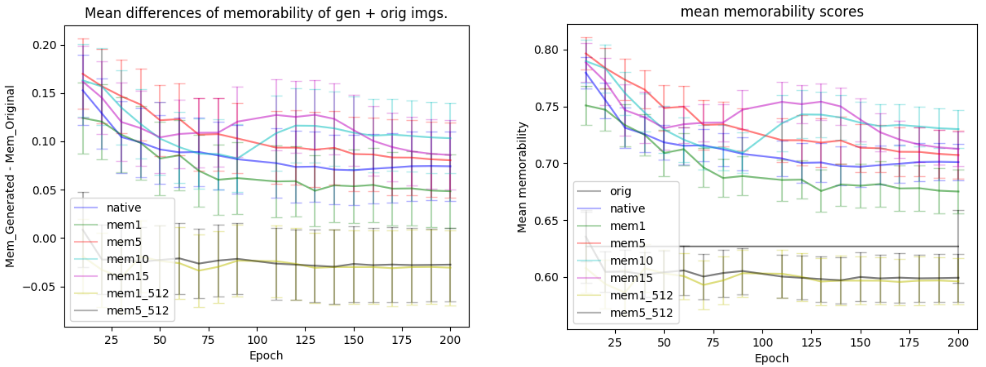
\includegraphics[width=\linewidth]{pic3.png}
    \caption{\textit{Showing stuff}}
\end{figure}

\begin{figure}
    \centering
    \label{pic3}
    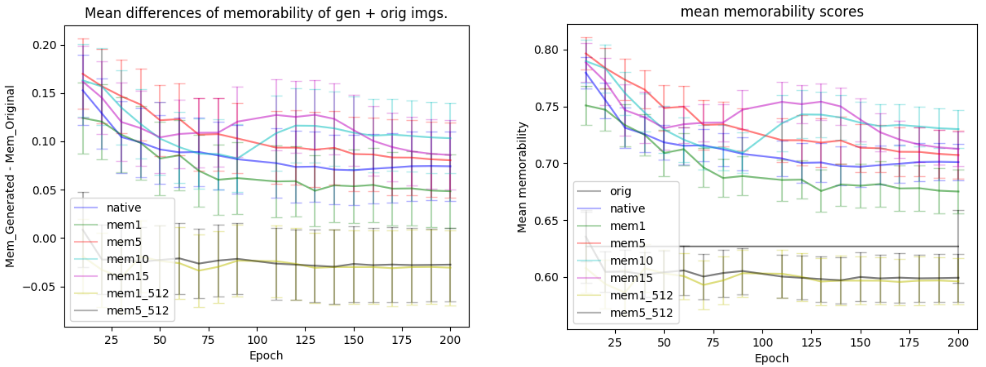
\includegraphics[width=\linewidth]{pic3.png}
    \caption{\textit{Showing stuff}}
\end{figure}

%%%%%%%%%%%%%%%%%%%%%%%%%%%%%%%%%%%%%%%%%%%%%%%%%%%%%%%%%%%%%%%%%%%%%%%%

Here we discuss the main successful results that we achieved throughout the course of this semester. We discuss graphs that show our concrete results, and we also show an experiment that we set up in order to gather human judgments on our generated images.

\subsection{Main results}

\subsection{Human opinion experiments}
Based on our experimental results, we asked several people to judge the images generated by our GAN. Although our original experiment hoped to generate images with increased memorability over the original inputted images, we decided to not ask our labelers to distinguish between these two. This is mainly due to the fact that low-resolution images tended to have noisy artifacts that would reveal the answer. Instead, we had humans distinguish between images generated by our MemGAN, and images generated by the native Pix2PixHD network. Each user had to judge between 100 pairs of images and identify which they found to be "more memorable," where each pair of images were generated by MemGAN and Pix2PixHD respectively (when fed in the same semantic map and original image). An example session is shown in Fig. \cite{}, where a user is given a pair of images to discern between for memorability. We gathered 1185 labels and found that 49.789\% of those labelings favored MemGAN as having generated the more memorable image. \\
% \noindent The original memorability experiments were designed 

% \begin{enumerate}
% \setlength{\itemsep}{1pt}
% \item Normal graphs and stuff
% \item Human opinion experiment results
% \end{enumerate}

\section{What did not work}
In this section, we describe a subset of experiments that did not perform as well as we had hoped.
\begin{enumerate}
\setlength{\itemsep}{1pt}
\item While the proposed loss worked well for 128x64 resolution, it failed to generalize to higher resolution such as 224x112, 512x256. 
\item Using MSELoss for the memorability loss
\item Scaling the gap parameter component of the loss.
\item Changing the resolution of the image passed to AMNet to obtain the memorability scores.
\item Removing perceptual loss and training only with memorability loss.
\end{enumerate}


\section{Future Work}
In future work, we hope to expand our method to work on higher-resolution images. Our results for low-resolution images seem promising given how the results matched our expectations in terms of visual effect alteration on the original images. We believe strongly that the task for low-resolution images is easier because of the comparatively smaller state space our network had for exploring higher-memorability images. With a smarter architecture, more computational resources, and additional experiments with other loss functions, we believe that generalizability for higher resolutions can be achieved so that we can more clearly visualize what our network has learned. These results seem promising and we hope to experiment more in the near future. \\
\indent Also, we would like to expand our work to focus on specific regions of an image. From results, we were able to observe that styles of specific objects in the scene were able to be manipulated, for example, car styles, and street markings on the ground. We would like to investigate how to inform the Pix2PixHD network to only manipulate certain regions of an image. Perhaps we wanted to train the network to only change the car's style over epochs and retain the other qualities of the image. This would allow shifting of focus of the image to certain regions of interest.
\indent Lastly, we hope to explore increasing other attributes of an image, such as making images more interesting, more beautiful, or more surprising. All of these attributes could be quantified using similar architectures as AMNet, and we see future work expanding MemGAN into other attributes as well. This work seems attainable given how our network was able to utilize memorability as an optimizable attribute; any arbitrary scalar that quantifies a desired attribute could have worked as well.\\


\section{Conclusion}
The results of this work suggests that memorability of an image can be increased, which is what we had sought to show at the beginning of the project. It shows some interesting changes in the more memorable images such contrast increase and lighting changes which also intuitively relates to memorability. The network is also able to change the style of specific elements in the image based on the semantic map (such as car styles, road markings, trees).  It also shows a framework that sees memorability as an attribute of an image, and can be used to increase any the presence of any attribute of an image, given that a classifier exists for that attribute -- and since memorability networks such as AMNet exists, this seems like a viable expansion to this work.




% \printbibliography 


%%%%%%%%%%%%%%%%%%%%%%%%%%%%%%%%%%%%%%%%%%%%%%%%%%%%


% Include other packages here, before hyperref.

% If you comment hyperref and then uncomment it, you should delete
% egpaper.aux before re-running latex.  (Or just hit 'q' on the first latex
% run, let it finish, and you should be clear).


{\small
\bibliographystyle{ieee}
\bibliography{egbib}
}

\end{document}
